\documentclass[11pt]{report}
\usepackage{times}
\usepackage{fullpage}
\usepackage{graphics}

%\usepackage{times}
\usepackage{listings}
\lstset{language=C,basicstyle=\footnotesize}

%\usepackage{tabularx}

\def\VERSION {0.4.0}
\def\HOMEPAGE {{\tt http://playerstage.sourceforge.net}}

\def\player {{\tt player}~}
\def\libgazebo {{\tt libgazebo}~}

\def\ahoward{Andrew Howard {\tt ahoward(at)usc.edu}}
\def\nkoenig{Nathan Koenig {\tt nkoenig(at)usc.edu}}
\def\srik{Srikanth Saripalli {\tt srik(at)usc.edu}}
\def\pranav{Pranav Srivastava {\tt pranav(at)seas.upenn.edu}}
\def\cvjones{Chris Jones {\tt cvjones(at)usc.edu}}
\def\mkobilar{Marin Kobilarov {\tt mkobilar(at)usc.edu}}
\def\sopheide{Stijn Opheide {\tt stijn.opheide(at)kotnet.org}}
\def\jmarien{Jef Marien {\tt jef.marien(at)student.kuleuven.ac.be}}
\def\kjans{Koen Jans {\tt koen.jans(at)student.kuleuven.ac.be}}
\def\ccote{Carle Cote {\tt Carle.Cote(at)USherbrooke.ca}}

\newcommand{\newinterface}[1]{\newpage \section{{\tt #1}}}
\newcommand{\newmodel}[2]{\def\modelName{#1} \newpage \section{{\tt #1}} \label{sec.model.#1} \subsection*{Authors} #2}

\begin{document}
\setcounter{page}{0}
\pagenumbering{roman}

%%%%%%%%%%%%%%%%%%%%%%%%%%%%%%%%%%%%%%%%%%%%%%%%%%%%%%%%%%%%%%%%%%%%%%%%%%%%%%%%%%%%
% Title page
%%%%%%%%%%%%%%%%%%%%%%%%%%%%%%%%%%%%%%%%%%%%%%%%%%%%%%%%%%%%%%%%%%%%%%%%%%%%%%%%%%%%

\titlepage

\begin{tabular}{lcr}
\begin{tabular}{c}
Player/Stage project\\
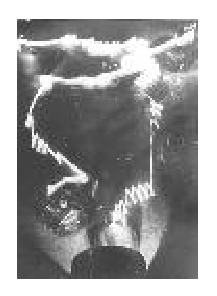
\includegraphics{notext_ps_logo}
\end{tabular}
&
\hspace{5cm}
&
\begin{tabular}{r}
{\bf USC Robotics Research Laboratory}\\
University of Southern California\\
Los Angeles, California, USA\\
\end{tabular}
\end{tabular}

\vspace{5cm}
\centerline{\huge{Gazebo}}
\vspace{0.5cm}
\centerline{\large{Version \VERSION\ User Manual}}
\vspace{2cm}

\centerline{\large Andrew Howard}
\centerline{\sl ahoward@usc.edu}
\vspace{0.5cm}
\centerline{\large Nathan Koenig}
\centerline{\sl nkoenig@usc.edu}

\vspace{5cm}
\centerline{\today}


%%%%%%%%%%%%%%%%%%%%%%%%%%%%%%%%%%%%%%%%%%%%%%%%%%%%%%%%%%%%%%%%%%%%%%%%%%%%%%%%%%%%
% Contents
%%%%%%%%%%%%%%%%%%%%%%%%%%%%%%%%%%%%%%%%%%%%%%%%%%%%%%%%%%%%%%%%%%%%%%%%%%%%%%%%%%%%

\newpage
\tableofcontents


%%%%%%%%%%%%%%%%%%%%%%%%%%%%%%%%%%%%%%%%%%%%%%%%%%%%%%%%%%%%%%%%%%%%%%%%%%%%%%%%%%%%
% Introduction
%%%%%%%%%%%%%%%%%%%%%%%%%%%%%%%%%%%%%%%%%%%%%%%%%%%%%%%%%%%%%%%%%%%%%%%%%%%%%%%%%%%%

\newpage
\setcounter{page}{0}
\pagenumbering{arabic}

\chapter{Introduction}

\section{What is Gazebo?}

Gazebo is a multi-robot simulator for outdoor environments.  Like
Stage, it is capable of simulating a population of robots, sensors and
objects, but does so in a three-dimensional world. It generates both
realistic sensor feedback and physically plausible interactions
between objects.

Gazebo is normally used in conjunction with the Player device server.
Player provides an abstracted, network-centric mechanism (a server)
through which robot controllers (clients) can interact with real
robots and sensors.  Gazebo works in conjunction with Player, providing
simulated sensor data in the place of real sensor data.  Ideally,
client programs cannot tell the difference between real devices and
the Gazebo simulation of those devices.

Gazebo can also be controlled through a low-level interface
(\libgazebo).  This library included to allow third-party developers
to easily integrate Gazebo into their own (non-Player) robot device
servers or architectures.

Last but not least, Player is Open Source and Free Software, released
under the GNU General Public License.  If you don't like how something
works, change it.  And please send us your patch!


\section{Stage and Gazebo}

The Player/Stage project provides two multi-robot simulators: Stage
and Gazebo.  Since Stage and Gazebo are both Player-compatible, client
programs written using one simulator can usually be run on the other
with little or no modification.  The key difference between these two
simulators is that whereas Stage is designed to simulate a very large
robot population with low fidelity, Gazebo is designed to simulated a
small population with high fidelity.  Thus, the two simulator are
complimentary, and users may switch back and forth between them
according to their needs.


\section{Getting Gazebo}

Gazebo is release in source form through the Player/Stage website:
\\\indent \HOMEPAGE\\
Check the downloads page for the latest software releases, and check
the documentation page for the latest version of this manual.


\section{System Requirements}

Gazebo is primarily developed for x86/Linux systems using GCC and GNU
autotools.  It can, however, be ported fairly easily to Posix-like
systems with X11 and OpenGL extensions (it is known to run
more-or-less out-of-the-box on Apple's OS X, for example).

For best performance, users should also ensure that they are using
hardware accelerated display drivers; try:
  \begin{verbatim}
  $ glxinfo \end{verbatim} %$ 
and check for ``direct rendering: Yes''.  Please, please don't ask the
Gazebo developers how to get hardware acceleration working for your
particular graphics card; you should be able to figure this out by
consulting various on-line sources.


\section{Bugs}

This software is provided WITHOUT WARRANTY.  Nevertheless, if you find
something that doesn't work, or there is some feature you would like
to see, you can submit a bug report/feature request through the
Player/Stage homepage:
\begin{quote} 
\HOMEPAGE
\end{quote}
Include a detailed description of you problem and/or feature request,
and information such as the Player version and operating system.  Make
sure you also select the ``gazebo'' category when reporting bugs.


\section{License}

This program is free software; you can redistribute it and/or modify
it under the terms of the GNU General Public License as published by
the Free Software Foundation; either version 2 of the License, or (at
your option) any later version.  This program is distributed in the
hope that it will be useful, but WITHOUT ANY WARRANTY; without even
the implied warranty of MERCHANTABILITY or FITNESS FOR A PARTICULAR
PURPOSE.  See the GNU General Public License for more details.  You
should have received a copy of the GNU General Public License along
with this program; if not, write to the Free Software Foundation,
Inc., 59 Temple Place - Suite 330, Boston, MA 02111-1307, USA.

\section{Acknowledgments}

Gazebo is written by Nate Koenig and Andrew Howard.  This work is
supported by DARPA grant DABT63-99-1-0015 (MARS).  Thanks also to
SourceForge.net for project hosting.


%%%%%%%%%%%%%%%%%%%%%%%%%%%%%%%%%%%%%%%%%%%%%%%%%%%%%%%%%%%%%%%%%%%%%%%%%%%%%%%%%%%%
% User Guide
%%%%%%%%%%%%%%%%%%%%%%%%%%%%%%%%%%%%%%%%%%%%%%%%%%%%%%%%%%%%%%%%%%%%%%%%%%%%%%%%%%%%

\part{User Guide}


%%%%%%%%%%%%%%%%%%%%%%%%%%%%%%%%%%%%%%%%%%%%%%%%%%%%%%%%%%%%%%%%%%%%%%%%%%%%%%%%%%%%
% General usage (quick start)
%%%%%%%%%%%%%%%%%%%%%%%%%%%%%%%%%%%%%%%%%%%%%%%%%%%%%%%%%%%%%%%%%%%%%%%%%%%%%%%%%%%%

\chapter{General Usage}

\section{Installing Third-Party Dependencies}

Gazebo relies on a number of third-party libraries, most of which will
probably be installed on your system by default.  You may, however,
have to install the following additional packages {\em before}
installing Gazebo:
\begin{itemize}
%
\item libXML2: pretty much all distributions will have this package.
%
\item OpenDynamicsEngine (ODE): most distributions have this package
(including RedHat, Gentoo, Fink); if in doubt, you can build it
yourself from the sources here:
\\ \indent http://opende.sourceforge.net/ode.html \\
%
\item Geospatial Data Abstraction Library (GDAL): this is less common,
although there is a Fink package.  Build it from the sources here:
\\ \indent http://remotesensing.org/gdal/ \\
\end{itemize}


\section{Building and Installing Gazebo}

The Gazebo source tarball can be obtained from
  \\ \indent http://playerstage.sourceforge.net/ \\
After unpacking the tarball, read the generic instructions in {\tt
README} and {\tt INSTALL}.  If you don't feel like reading those
files, the following should suffice in most cases:
\begin{verbatim}
  $ ./configure
  $ make
  $ make install
\end{verbatim} %$
Gazebo will be installed in the default location: {\tt /usr/local/}.
The {\tt configure} script accepts a number of options for customizing
the build process, including changing the install location and
adding/removing device drivers.  For example, to change the install
location for Gazebo to \verb+~/local+ in your home directory, use:
\begin{verbatim}
  $ ./configure --prefix /home/<username>/local
\end{verbatim} %$
Please read the FAQ entry on local installations, available here:
\\ \indent http://playerstage.sourceforge.net/faq.html\\

To see a complete list of build options, use:
\begin{verbatim}
  $ ./configure --help
\end{verbatim} %$
If you are going to use Gazebo with Player, note that Gazebo must be
installed {\em before} Player.


\section{Starting Gazebo}

The Gazebo server can be started as follows:
\begin{verbatim}
  $ gazebo <worldfile>
\end{verbatim} %$
where \verb+<worldfile>+ is the file containing the description of the
world and everything in it.  Sample world files can be found in the
{\tt worlds} directory of the source distribution, or in the
installed version under {\tt /usr/local/share/gazebo/worlds/}
(default install).  For example:
\begin{verbatim}
  $ gazebo /usr/local/share/gazebo/worlds/example1.world
\end{verbatim} %$
will create a simple world with a single robot.  Gazebo will display a
window with a view of the simulated world; the camera viewpoint can be
changed by dragging around with the mouse.


\section{Working with Player}

The Player device server treats Gazebo in exactly the same way that it
treats real robot hardware: as a device that is a source of data and a
sink for commands.  Users must therefore run Player seperately, and
point it at an running instance of Gazebo.  Player has a number of
specific drivers, such as {\tt gz\_position} and {\tt gz\_laser} that
can be used to interact with Gazebo models.

For example, after starting Gazebo as per the above example, run
Player like this:
\begin{verbatim}
  $ player -g default /usr/local/share/player/config/gazebo.cfg
\end{verbatim} %$
Player will output a message indicating that is has connected with the
simulation:
\begin{verbatim}  
   libgazebo msg : opening /tmp/gazebo-<username>-default-sim-default
\end{verbatim} %$
Users can now interact with the simulated robot exactly as the would a
real robot.  Try running {\tt playerv}, for example:
\begin{verbatim}  
  $ playerv --position:0 --laser:0
\end{verbatim} %$
This will pop up the standard Player viewer utility.  You should see
an outline of the robot and the laser scan.  Use the mouse to pan and
zoom.  You can driver the robot around by selecting the "command" option
from the menu, and then dragging the little cross hairs to where you
want the robot to go.  You should see the the robot in the Gazebo window
moving at the same time.

See Chapter \ref{sec.player} for examples of typical Player/Gazebo
configurations, and consult the Player manual for information on
specific Player drivers.


\section{Command Line Options}
\label{sec.cmdline}

Gazebo recognizes the following command line options.
\begin{center}
\begin{tabular}{|cl|}
\hline
\bf Argument & \bf Meaning \\ 
\hline
-v & Print the version string. \\
\hline
\end{tabular}
\end{center}



%%%%%%%%%%%%%%%%%%%%%%%%%%%%%%%%%%%%%%%%%%%%%%%%%%%%%%%%%%%%%%%%%%%%%%%%%%%%%%%%%%%%
% World file
%%%%%%%%%%%%%%%%%%%%%%%%%%%%%%%%%%%%%%%%%%%%%%%%%%%%%%%%%%%%%%%%%%%%%%%%%%%%%%%%%%%%

\newenvironment{xmlattrtable}[2]
  {\begin{center}\begin{tabular}{llll} \multicolumn{4}{c}{{\bf $<$#1:#2$>$}}\\ 
    \hline Attribute & Type & Default & Description \\ \hline}
  {\hline \end{tabular}\end{center}}

\newcommand{\xmlattr}[4]{{\tt $<$#1$>$} & #2 & #3 & #4\\} 
\newcommand{\modeldefaults}{
  \xmlattr{id}{string}{NULL}{Model ID string}
  \xmlattr{xyz}{3-vector}{$(0, 0, 0)$}{Model position}
  \xmlattr{rpy}{Euler angles}{$(0, 0, 0)$}{Model orientation}}


\newenvironment{bodyattrtable}
  {\begin{center}\begin{tabular}{lll}  
    \hline Name & Description \\ \hline}
  {\hline \end{tabular}\end{center}}

\newcommand{\bodyattr}[2]{{\tt #1} & #2\\} 
\newcommand{\bodydefaults}{
  \bodyattr{canonical}{The canonical (default) body.}}



\chapter{The World File}
\label{sec.worldfile.ref}

The world file contains a description of the world to be simulated by
Gazebo.  It describes the layout of robots, sensors, light sources,
user interface components, and so on.  The world file can also be used
to control some aspects of the simulation engine, such as the force of
gravity or simulation time step.

Gazebo world files are written in XML, and can thus be created and
modified using a text editor.  Sample world files can be found in the
{\tt worlds} directory of the source distribution, or in the installed
version (default install) under 
\\ \indent {\tt /usr/local/share/gazebo/worlds/} \\


\section{Key Concepts and Basic Syntax}

The world consists mainly of {\em model} declarations.  A model can be
a robot (e.g. a Pioneer2AT or SegwayRMP), a sensor (e.g. SICK LMS200),
a static feature of the world (e.g. MapExtruder) or some manipulable
object.  
%
For example, the following declaration will create a Pioneer2AT named
``{\tt robot1}'':
\begin{verbatim}
  <model:Pioneer2AT>
    <id>robot1</id>
    <xyz>0 0 0.40</xyz>
    <rpy>0 0 45</rpy>
  </model:Pioneer2AT>
\end{verbatim}
Associated with each model is a set of {\em attributes} such as the
model's position {\tt <xyz>} and orientation {\tt <rpy>}; see Section
\ref{sec.model.ref} for a complete list of models and their
attributes.

Models can also be composed.  One can, for example, attach a scanning
laser range-finder to a robot:
\begin{verbatim}
  <model:Pioneer2AT>
    <id>robot1</id>
    <xyz>0 0 0.40</xyz>
    <rpy>0 0 45</rpy>
    <model:SickLMS200>
      <id>laser1</id>
      <parentBody>chassis</parentBody>
      <xyz>0.15 0 0.20</xyz>
      <rpy>0 0 0</rpy>
    </model:SickLMS200>
  </model:Pioneer2AT>
\end{verbatim}
The {\tt <parentBody>} tag indicates which part of the robot the laser
should be attached to (in this case, the chassis rather than the
wheels).  The {\tt <xyz>} and {\tt <rpy>} tags describe the laser's
position and orientation with respect to this body (see Section
\ref{sec.world.units} for a discussion of coordinate systems).  Once
attached, robot and the laser form a single rigid body.


\section{Graphical User Interface}

While Gazebo can operate without a GUI, it is often useful to have a
viewport through which the user can inspect the world.  In Gazebo,
such user interface components are provided through special models
(such as the {\tt ObserverCam}) that can be declared and configured in
the world file.  See the documentation on the {\tt ObserverCam} model
for details.


\section{Canonical World File Layout}

The ``standard'' layout for the world file is can be seen from the
examples included in the {\tt worlds} directory.  The basic components
are as follows:

\begin{itemize}
%
\item XML meta-data, start of world block, more XML meta-data:
\begin{verbatim}
  <?xml version="1.0"?>
  <gz:world 
    xmlns:gz='http://playerstage.sourceforge.net/gazebo/xmlschema/#gz'
    ...
\end{verbatim}
%
\item Global parameters:
\begin{verbatim}
    <params:GlobalParams>
      <gravity>0.0 0.0 -9.8</gravity>
    </params:GlobalParams>
\end{verbatim}
%
\item GUI components:
\begin{verbatim}
    <model:ObserverCam>
      <id>userCam0</id>
      <xyz>0.504 -0.735 0.548</xyz>
      <rpy>-0 19 119</rpy>
      <window>
        <title>Observer</title>
        <size>640 480</size>
        <pos>0 0</pos>
      </window>
    </model:ObserverCam>
\end{verbatim}
%
\item Light sources (without lights, the scene will be very dark):
\begin{verbatim}
    <model:LightSource>
      <id>light0</id>
      <xyz>0.0 0.0 10.0</xyz>
    </model:LightSource>
\end{verbatim}
%
\item Ground planes and/or terrains:
\begin{verbatim}
    <model:GroundPlane>
      <id>ground1</id>
    </model:GroundPlane>
\end{verbatim}
%
\item Robots, objects, etc.:
\begin{verbatim}
    <model:Pioneer2AT>
      <id>robot1</id>
      <xyz>0 0.0 0.5</xyz>
      <model:SickLMS200>
        <id>laser1</id>
        <xyz>0.15 0 0.20</xyz>
      </model:SickLMS200>
    </model:Pioneer2AT>
\end{verbatim}
%
\item End of world block:
\begin{verbatim}
  </gz:world>
\end{verbatim}
\end{itemize}
%
A detailed list of models and their attributes can be found in
Chapters \ref{sec.nonmodel.ref} and \ref{sec.model.ref}.


\section{Coordinate Systems and Units}
\label{sec.world.units}

% Coordinate systems
By convention, Gazebo uses a right-handed coordinate system, with $x$
and $y$ in the plane, and $z$ increasing with altitude.  Most models
are designed such that the are upright (with respect to the $z$ axis)
and pointing along the positive $x$ axis.  The tag {\tt <xyz>} is used
to indicate an object's position ($x$, $y$ and $z$ coordinates); the
tag {\tt <rpy>} is used to indicate an objects orientation (Euler
angles; i.e., roll, pitch and yaw).
%
For example, {\tt <xyz>1 2 3</xyz>} indicates a translation of 1~m
along the x-axis, 2~m along the y-axis and 3~m along the z-axis; {\tt
<rpy>10 20 30</rpy>} indicates a rotation of 30~degrees about the
z-axis (yaw), followed by a rotation pf 20~degrees about the y-axis
(pitch) and a rotation of 10~degrees about the x-axis (roll).

% Units
Unless otherwise specified, the world file uses SI units (meters,
seconds, kilograms, etc).  The following idioms should also be noted:
\begin{itemize}
\item Angles and angular velocities are measured in degrees and
degrees/sec, respectively.
\end{itemize}


%%%%%%%%%%%%%%%%%%%%%%%%%%%%%%%%%%%%%%%%%%%%%%%%%%%%%%%%%%%%%%%%%%%%%%%%%%%%%%%%%%%%
% Player
%%%%%%%%%%%%%%%%%%%%%%%%%%%%%%%%%%%%%%%%%%%%%%%%%%%%%%%%%%%%%%%%%%%%%%%%%%%%%%%%%%%%



%%%%%%%%%%%%%%%%%%%%%%%%%%%%%%%%%%%%%%%%%%%%%%%%%%%%%%%%%%%%%%%%%%%%%%%%%%%%%%%%%%%%
% Player
%%%%%%%%%%%%%%%%%%%%%%%%%%%%%%%%%%%%%%%%%%%%%%%%%%%%%%%%%%%%%%%%%%%%%%%%%%%%%%%%%%%%

\chapter{Working with Player}
\label{sec.player}

The Player device server treats Gazebo in exactly the same way that it
treats real robot hardware: as a device that is a source of data and a
sink for commands.  A key advantage of this approach is that users may
mix Player {\em abstract} drivers with simulation drivers.  Thus, for
example, drivers such as VFH (Vector Field Histogram) and AMCL
(adapative Monte-Carlo localization), will work equally well with
simulated and real robots.  In the following sections, we describe
some basic scenarios that demonstate this interaction.

\section{Setting up the Simulation}

The basic steps for setting up and running a combined Player/Gazebo
simulation are as follows.
\begin{enumerate}
\item Write the Gazebo world file.
\item Start Gazebo.
\item Write the corresponding Player configuration file(s).
\item Start Player(s).
\item Start client program(s).
\end{enumerate}
Note that Gazebo must be started {\em before} the Player server, and
that the Player server must {\em re-started} whenever Gazebo is
re-started.


\section{Example: Using a Single Robot}

Consider the case of a single robot with a scanning laser
range-finder.  The following Gazebo world file snippet will create a
Pioneer2DX robot with SICK~LMS200 laser.
\begin{verbatim}
  <model:Pioneer2DX>
    <id>robot1_position</id>
    <xyz>0 0 0.40</xyz>
    <rpy>0 0 45</rpy>
    <model:SickLMS200>
      <id>robot1_laser</id>
      <xyz>0.15 0 0.20</xyz>
      <rpy>0 0 0</rpy>
    </model:SickLMS200>
  </model:Pioneer2DX>
\end{verbatim}
The corresponding snippet of the Player configuration file should look
like this:
\begin{verbatim}
  position:0
  (
    driver "gz_position"
    gz_id "robot1_position"
  )

  laser:1
  (
    driver "gz_laser"
    gz_id "robot1_laser"
  )
\end{verbatim}

To run this simulation, start Gazebo with:
\begin{verbatim}
  $ gazebo <myworld>
\end{verbatim} %$
where \verb+<myworld>+ is the name of the Gazebo world file,
and start Player with
\begin{verbatim}
  $ player -g default <myconfig>
\end{verbatim} %$
where \verb+<myconfig>+ is the name of the Player configuration file.
%
Client programs can connect to the simulated devices devices on the
default Player port 6665.


\section{Example: Using a Single Robot with the VFH driver}

Abstract devices can be mixed freely with simulated devices in the
Player server.  Thus, for example, it is possible to use the VFH
(Vector Field Histogram) driver with a simulated robot.  The following
Gazebo world file snippet will create a Pioneer2DX robot with
SICK~LMS200 laser.
\begin{verbatim}
  <model:Pioneer2DX>
    <id>robot1_position</id>
    <xyz>0 0 0.40</xyz>
    <rpy>0 0 45</rpy>
    <model:SickLMS200>
      <id>robot1_laser</id>
      <xyz>0.15 0 0.20</xyz>
      <rpy>0 0 0</rpy>
    </model:SickLMS200>
  </model:Pioneer2DX>
\end{verbatim}
The corresponding snippet of the Player configuration file should look
like this:
\begin{verbatim}
  position:0
  (
    driver "gz_position"
    gz_id "robot1_position"
  )

  laser:0
  (
    driver "gz_laser"
    gz_id "robot1_laser"
  )

  position:1
  (
    driver "vfh"
    <vfh driver settings>
  )
\end{verbatim}
Note that the configuration file is exactly as per the first example;
we have simply added another device to the Player server.  The VFH
driver will use the simulated robot chassis and laser exactly as it
would a real robot chassis and laser.

To run this simulation, start Gazebo with:
\begin{verbatim}
  $ gazebo <myworld>
\end{verbatim} %$
where \verb+<myworld>+ is the name of the Gazebo world file,
and start Player with
\begin{verbatim}
  $ player -g default <myconfig>
\end{verbatim} %$
where \verb+<myconfig>+ is the name of the Player configuration file.
%
Client programs can connect to the server on the default Player port
6665.


\section{Example: Using Multiple Robots}

There are a number of ways to work with multiple robots.  The simplest
way is to use multiple instances of the Player server (one for each
robot being simulated).
%
The following Gazebo world file snippet will create a pair of
Pioneer2DX robots with SICK~LMS200 lasers.
\begin{verbatim}
  <model:Pioneer2DX>
    <id>robot1_position</id>
    <xyz>0 0 0.40</xyz>
    <rpy>0 0 45</rpy>
    <model:SickLMS200>
      <id>robot1_laser</id>
      <xyz>0.15 0 0.20</xyz>
      <rpy>0 0 0</rpy>
    </model:SickLMS200>
  </model:Pioneer2DX>

  <model:Pioneer2DX>
    <id>robot2_position</id>
    <xyz>0 0 0.40</xyz>
    <rpy>0 0 45</rpy>
    <model:SickLMS200>
      <id>robot2_laser</id>
      <xyz>0.15 0 0.20</xyz>
      <rpy>0 0 0</rpy>
    </model:SickLMS200>
  </model:Pioneer2DX>
\end{verbatim}
Since there will be two instances of the Player server, two different
configuration files are required.   For the first robot:
\begin{verbatim}
  position:0
  (
    driver "gz_position"
    gz_id "robot1_position"
  )

  laser:1
  (
    driver "gz_laser"
    gz_id "robot1_laser"
  )
\end{verbatim}
and for the second robot:
\begin{verbatim}
  position:0
  (
    driver "gz_position"
    gz_id "robot2_position"
  )

  laser:1
  (
    driver "gz_laser"
    gz_id "robot2_laser"
  )
\end{verbatim}
Note that these files are identical apart from the \verb+gz_id+
property.  In general, however, the simulated robots may be
heterogeneous, in which case the Player configuration files will
differ substantially.

To run this simulation, start Gazebo with:
\begin{verbatim}
  $ gazebo <myworld>
\end{verbatim} %$
where \verb+<myworld>+ is the name of the Gazebo world file,
and start two instances of Player with
\begin{verbatim}
  $ player -p 7000 -g default <myconfig1>
\end{verbatim} %$
and
\begin{verbatim}
  $ player -p 7001 -g default <myconfig2>
\end{verbatim} %$
where \verb+<myconfig1>+ and \verb+<myconfig2>+ are the two Player
configuration files.
%
Client programs can connect to the robots \verb+robot1+ and
\verb+robot2+ through ports 7000 and 7001, respectively.



\section{Example: Using Multiple Robots with {\tt --gazebo-prefix}}

When the simulated robots are homogeneous, one may simplify the
process somewhat by employing the \verb+--gazebo-prefix+ flag with
Player.
%
The following Gazebo world file snippet will create a pair of
Pioneer2DX robots with SICK~LMS200 lasers.
\begin{verbatim}
  <model:Pioneer2DX>
    <id>robot1_position</id>
    <xyz>0 0 0.40</xyz>
    <rpy>0 0 45</rpy>
    <model:SickLMS200>
      <id>robot1_laser</id>
      <xyz>0.15 0 0.20</xyz>
      <rpy>0 0 0</rpy>
    </model:SickLMS200>
  </model:Pioneer2DX>

  <model:Pioneer2DX>
    <id>robot2_position</id>
    <xyz>0 0 0.40</xyz>
    <rpy>0 0 45</rpy>
    <model:SickLMS200>
      <id>robot2_laser</id>
      <xyz>0.15 0 0.20</xyz>
      <rpy>0 0 0</rpy>
    </model:SickLMS200>
  </model:Pioneer2DX>
\end{verbatim}
Since the robots are identical, we can write one Player configuration
file for both:
\begin{verbatim}
  position:0
  (
    driver "gz_position"
    gz_id "_position"
  )

  laser:1
  (
    driver "gz_laser"
    gz_id "_laser"
  )
\end{verbatim}
Note that the \verb+gz_id+ values are incomplete; we will add {\em
prefix} to these values when the Player server is started.

To run this simulation, start Gazebo with:
\begin{verbatim}
  $ gazebo <myworld>
\end{verbatim} %$
where \verb+<myworld>+ is the name of the Gazebo world file,
and start two instances of Player with
\begin{verbatim}
  $ player -p 7000 -g default --gazebo-prefix robot1 <myconfig>
\end{verbatim} %$
and
\begin{verbatim}
  $ player -p 7001 -g default --gazebo-prefix robot 2 <myconfig>
\end{verbatim} %$
where \verb+<myconfig>+ is the common Player configuration file.
%
Client programs can connect to the robots \verb+robot1+ and
\verb+robot2+ through ports 7000 and 7001, respectively.






%%%%%%%%%%%%%%%%%%%%%%%%%%%%%%%%%%%%%%%%%%%%%%%%%%%%%%%%%%%%%%%%%%%%%%%%%%%%%%%%%%%%
% Model reference
%%%%%%%%%%%%%%%%%%%%%%%%%%%%%%%%%%%%%%%%%%%%%%%%%%%%%%%%%%%%%%%%%%%%%%%%%%%%%%%%%%%%

\chapter{Non-model Reference}
\label{sec.nonmodel.ref}

\section{Global Paramamerters}

General parameters used by Gazebo.

\begin{xmlattrtable}{params}{GlobalParams}
\xmlattr{gravity}{3-vector}{(0,0,-9.8)}{Gravity vector}
\end{xmlattrtable}


%%%%%%%%%%%%%%%%%%%%%%%%%%%%%%%%%%%%%%%%%%%%%%%%%%%%%%%%%%%%%%%%%%%%%%%%%%%%%%%%%%%%
% Model reference
%%%%%%%%%%%%%%%%%%%%%%%%%%%%%%%%%%%%%%%%%%%%%%%%%%%%%%%%%%%%%%%%%%%%%%%%%%%%%%%%%%%%

\chapter{Model Reference}
\label{sec.model.ref}

Gazebo currently supports the following models.
\begin{itemize}
\item {\tt AvatarHeli}: USC AVATAR Helicopter.
\item {\tt Blimp}: A dirigible.
\item {\tt ClodBuster}: Car-like Non-Holonomic 4-wheeled Robot with Ackerman Steering.
\item {\tt Factory}: A tool to dynamically create models.
\item {\tt GarminGPS}: Basic GPS device model. 
\item {\tt GroundPlane}: A flat plane that represents the ground.
\item {\tt LightSource}: A single point light.
\item {\tt MapExtruder}: Linearly extrudes a 2D image into 3D geometry.
\item {\tt ObserverCam}: A gods-eye camera (GUI component for user interaction).
\item {\tt Pioneer2AT}: ActivMedia Pioneer2AT (``all terrain'')
robot with 4 wheels and skid steering.
\item {\tt Pioneer2DX}: ActivMedia Pioneer2DX (indoor)
robot with 2 drive wheels and a castor.
\item {\tt Pioneer2Gripper}: ActivMedia Pioneer2 Gripper.
\item {\tt Pioneer2Sonars}: ActivMedia Pioneer2 sonar ring.
\item {\tt PointSet}: A model to visualize a point cloud.
\item {\tt SegwayRMP}: custom modified Segway RMP (``Robot Mobility
Platform'') robot.
\item {\tt SickLMS200}: the ubiquitous SICK scanning laser
range-finder.
\item {\tt Shrimp}: A robot designed after the Shrimp robot by BlueBotics.
\item {\tt SimpleSolid}: Simple solid shapes, such as boxes and spheres.
\item {\tt SonyVID30}: color video camera with controllable
pan-tilt-zoom.
\item {\tt Terrain}: A terrain triangle mesh model.
\item {\tt TotemPole}: A vertical pole of simple solids, used as a visual fiducial.
\item {\tt TruthWidget}: A magical device for getting and seting model poses.
\item {\tt WheelChair}: A wheelchair robot.
\end{itemize}

\newmodel{AvatarHeli}{\srik}

\subsection{Overview}

The {\tt AvatarHeli} model simulates the USC AVATAR helicopter, a Bergen Industrial Twin RC helicopter (http://www.bergenrc.com/IndustrialTwin.asp).

\subsection{\libgazebo Interfaces}

{\tt AvatarHeli} currently does not support any interfaces. 


\subsection{Player Drivers}

No player drivers are available.

\subsection{World File Attributes}

{\tt AvatarHeli} models can be instantiated using the
\verb+<model:AvatarHeli>+ tag.  The following attributes are
supported.

\begin{xmlattrtable}{model}{AvatarHeli}
\modeldefaults
\end{xmlattrtable}


\subsection{Body Attributes}

The following bodies are used by this model.

\begin{bodyattrtable}
\bodydefaults
\end{bodyattrtable}


\newmodel{Blimp}{\pranav}

\subsection{Overview}

The {\tt Blimp} model simulates a UPenn Blimp. 

\subsection{\libgazebo Interfaces}

{\tt Blimp} supports the \libgazebo {\tt position} and {\tt position3d} interface.

\subsection{Player Drivers}

Basic motor control and odometry information is available through the
{\tt gz\_position} or {\tt gz\_position3d} driver.


\subsection{World File Attributes}

{\tt Blimp} models can be instantiated using the
\verb+<model:Blimp>+ tag.  The following attributes are
supported.

\begin{xmlattrtable}{model}{Blimp}
\modeldefaults
\xmlattr{is3d}{true/false}{false}{Does this use the position3d interface?}
\end{xmlattrtable}

\subsection{Body Attributes}

The following bodies are used by this model.

\begin{bodyattrtable}
\bodydefaults
\end{bodyattrtable}


\newmodel{ClodBuster}{\pranav}

\subsection{Overview}

The {\tt ClodBuster} model simulates the UPenn ClodBuster robot (4 wheel
drive robot with Ackerman steering).

\subsection{\libgazebo Interfaces}

{\tt ClodBuster} supports the \libgazebo {\tt position} interface.


\subsection{Player Drivers}

Basic motor control and odometry information is available through the
{\tt gz\_position} driver.


\subsection{World File Attributes}

{\tt ClodBuster} models can be instantiated using the
\verb+<model:ClodBuster>+ tag.  The following attributes are
supported.

\begin{xmlattrtable}{model}{ClodBuster}
\modeldefaults
\xmlattr{raw\_encoder\_position}{true/false}{false}{Flag indicating return of raw wheel encoder values.}
\end{xmlattrtable}

\subsection{Body Attributes}

The following bodies are used by this model.

\begin{bodyattrtable}
\bodydefaults
%\bodyattr{tires}{The four tires}
%\bodyattr{stubs}{Blocks attaching the tires to the main body}
\end{bodyattrtable}


\newmodel{Factory}{\cvjones, \nkoenig}

\subsection{Overview}

The {\tt Factory} model maintains no physical characteristics, but instead
allows the user to dynamically create models at runtime. A model is
instantiated by passing an XML character string to a {\tt Factory} model.
The character string use the same model format as the .world files. Note
that the string should {\em only} contain the model description, and no
other tags. The XML string is passed into Gazebo through the gz\_factory
interface which has the same interface as the Player speech device.  

\subsection{\libgazebo Interfaces}

{\tt Factory} supports the \libgazebo {\tt factory} interface.


\subsection{Player Drivers}

A new model is created using the {\tt gz\_factory} driver.

\subsection{World File Attributes}

{\tt Factory} models can be instantiated using the \verb+<model:Factory>+
tag. The following attributes are supported.

\begin{xmlattrtable}{model}{Factory}
\xmlattr{id}{string}{NULL}{Model ID string}
\end{xmlattrtable}


\subsection{Body Attributes}

This model does not have a physical representation.


\newmodel{GarminGPS}{\pranav}

\subsection{Overview}

The {\tt \modelName} model simulates GPS information by using the
flat-world approximation.  It doesn't account for GPS occlusion or
loss of signal, etc.

\subsection{\libgazebo Interfaces}

{\tt \modelName} supports the \libgazebo {\tt gps} interfaces.

\subsection{Player Drivers}

The GPS position are available through the {\tt gz\_gps} driver. 

\subsection{World File Attributes}

{\tt \modelName} models can be instantiated using the
\verb+<model:GarminGPS>+ tag.  The following attributes are
supported.

\begin{xmlattrtable}{model}{\modelName}
\modeldefaults
\xmlattr{origin}{3-vector}{(0,0,0)}{coordinates of the origin in lat-long-alt}
\end{xmlattrtable}

\subsection{Body Attributes}

The following bodies are used by this model.

\begin{bodyattrtable}
\bodydefaults
\end{bodyattrtable}


\newmodel{GroundPlane}{\nkoenig}
\subsection{Overview}

The {\tt \modelName} model simulates a flat infinite plane.

\subsection{\libgazebo Interfaces}

{\tt \modelName} has no \libgazebo interface.

\subsection{Player Drivers}

There are no player drivers.

\subsection{World File Attributes}

{\tt \modelName} models can be instantiated using the
\verb+<model:GroundPlane>+ tag.  The following attributes are
supported.

\begin{xmlattrtable}{model}{\modelName}
\modeldefaults
\xmlattr{normal}{3-vector}{(0,0,1)}{Direction of the normal vector}
\xmlattr{height}{double}{0}{Distance along the z-axis to place the plane}
\xmlattr{color}{3-vector}{(0,0,0)}{RGB color}
\xmlattr{texture2D}{string}{NULL}{Texture image filename}
\xmlattr{cfm}{double}{0.01}{Constraint Force Mixing parameter}
\end{xmlattrtable}


\subsection{Body Attributes}

The following bodies are used by this model.

\begin{bodyattrtable}
\bodydefaults
\end{bodyattrtable}



\newmodel{LightSource}{\ahoward, \nkoenig}


\subsection{Overview}

The {\tt LightSource} model simulates a single point light.

\subsection{\libgazebo Interfaces}

{\tt LightSource} has no \libgazebo interface.

\subsection{Player Drivers}

There are no player drivers.

\subsection{World File Attributes}

{\tt LightSource} models can be instantiated using the
\verb+<model:LightSource>+ tag.  The following attributes are
supported.

\begin{xmlattrtable}{model}{LightSource}
\modeldefaults
\xmlattr{ambientColor}{4-vector}{(0.2 0.2 0.2 1.0)}{Ambient color}
\xmlattr{diffuseColor}{4-vector}{(0.8 0.8 0.8 1.0)}{Diffuse color}
\xmlattr{specularColor}{4-vector}{(0.2 0.2 0.2 1.0)}{Specular color}
\xmlattr{attenuation}{3-vector}{(1.0 0.0 0.0)}{Constant, Linear, Quadratic attenuation}

\end{xmlattrtable}

\subsection{Body Attributes}

The following bodies are used by this model.
\begin{bodyattrtable}
\bodydefaults
\end{bodyattrtable}


\newmodel{MapExtruder}{\nkoenig}


\subsection{Overview}

The {\tt MapExtruder} model extrudes a 2D image into 3D geometry. This
is useful for generating simple maps.  The bottom left point in the
image is mapped to the position specified by the {\tt pos} tag.

\subsection{\libgazebo Interfaces}

{\tt MapExtruder} currently has no \libgazebo interface.


\subsection{Player Drivers}

There are no player drivers.

\subsection{World File Attributes}

{\tt MapExtruder} models can be instantiated using the
\verb+<model:MapExtruder>+ tag.  The following attributes are
supported.

\begin{xmlattrtable}{model}{MapExtruder}
\modeldefaults
\xmlattr{imageFile}{string}{NULL}{PPM image file to extrude}
\xmlattr{negative}{true/false}{false}{Use the inverse color values}
\xmlattr{threshold}{integer}{200}{Value over which a pixel is considered filled space}
\xmlattr{width}{float}{0.1}{Width of the geometries}
\xmlattr{height}{float}{1}{Height of the geometries, along z-axis}
\xmlattr{scale}{float}{0.1}{Scale the map up or down}
\xmlattr{color}{3-vector}{(0,0,0)}{RGB color}
\xmlattr{errBound}{float}{5}{Allowable error in the geometries}
\xmlattr{halign}{left/center}{left}{Horizontal alignment}
\xmlattr{valign}{bottom/center}{bottom}{Vertical alignment}

\end{xmlattrtable}


\subsection{Body Attributes}

The following bodies are used by this model.

\begin{bodyattrtable}
\bodydefaults
\end{bodyattrtable}




\newmodel{ObserverCam}{\nkoenig, \ahoward}

\subsection{Overview}

The {\tt \modelName } model provides a interactive viewport through
which users can view the simulation (think of it as a fly god's eye).

\subsection{World File Attributes}

{\tt \modelName} models can be instantiated using the
\verb+<model:ObserverCam>+ tag.  The following attributes are
supported.

\begin{xmlattrtable}{model}{\modelName}
\modeldefaults
\xmlattr{updatePeriod}{float}{0.1}{Seconds between refresh}
\xmlattr{displayRays}{true/false}{false}{Display laser rays}
\xmlattr{saveFrames}{string}{NULL}{Directory to store image frames}
\xmlattr{shadeModel}{flat/smooth}{flat}{OpenGL shading model}
\xmlattr{polygonMode}{point/line/fill}{fill}{OpenGL polygon mode}
\xmlattr{lens}{}{}{Camera lens attributes}
~~~~\xmlattr{hfov}{degrees}{60}{Horizontal field of view}
~~~~\xmlattr{nearClip}{meters}{0.20}{Distance to near clip plane}
~~~~\xmlattr{farClip}{meters}{1000.0}{Distance to far clip plane}

\end{xmlattrtable}

\subsection{Windows}

The following are definitions for the {\tt ObserverWindow}. The window attribute block must be a child of {\bf$<$model:\modelName$>$}. 

\begin{xmlattrtable}{window}{X11GLWindow}
\xmlattr{id}{string}{NULL}{Window ID string}
\xmlattr{title}{string}{NULL}{Window title string}
\xmlattr{size}{2-vector}{(100,100)}{Initial size of the window}
\xmlattr{moveScale}{float}{0.1}{Mouse movement scale factor}
\end{xmlattrtable}


\begin{center}
\begin{tabular}{|c|c|c|}
\multicolumn{3}{c}{\bf Mouse Commands} \\
\hline
\bf Button & \bf Vertical Move & \bf Horizontal Move \\
\hline
Left & Rotate along X axis & Rotate along Z axis \\
\hline
Middle & Translate along Z axis & Translate along X axis \\
\hline
Right & Translate along Y axis & Translate along X axis \\
\hline
\end{tabular}
\end{center}


\subsection{Body Attributes}

This model does not have a physical representation.



\newmodel{Pioneer2AT}{\ahoward, \nkoenig}

\subsection{Overview}

The {\tt \modelName} model simulates the ActivMedia Pioneer2AT (``all
terrain'') robot with 4 wheels and skid steering.  Currently, it does
not simulate the robot's sonar ring.


\subsection{\libgazebo Interfaces}

{\tt \modelName} supports the \libgazebo {\tt position} interface.


\subsection{Player Drivers}

Basic motor control and odometry information is available through the
{\tt gz\_position} driver.


\subsection{World File Attributes}

{\tt \modelName} models can be instantiated using the
\verb+<model:Pioneer2AT>+ tag.  The following attributes are
supported.

\begin{xmlattrtable}{model}{\modelName}
\modeldefaults
\end{xmlattrtable}


\subsection{Body Attributes}

The following bodies are used by this model.

\begin{bodyattrtable}
\bodydefaults
%\bodyattr{chassis}{The Pioneer chassis}
\end{bodyattrtable}


\newmodel{Pioneer2DX}{\ahoward}

\subsection{Overview}

The {\tt \modelName} model simulates the ActivMedia Pioneer2DX
(indoor) robot with 2 drive wheels and a castor.  Currently, it does
not simulate the robot's sonar ring.


\subsection{\libgazebo Interfaces}

{\tt \modelName} supports the \libgazebo {\tt position} interface.


\subsection{Player Drivers}

Basic motor control and odometry information is available through the
{\tt gz\_position} driver.


\subsection{World File Attributes}

{\tt \modelName} models can be instantiated using the
\verb+<model:Pioneer2DX>+ tag.  The following attributes are
supported.

\begin{xmlattrtable}{model}{\modelName}
\modeldefaults
\end{xmlattrtable}

\subsection{Body Attributes}

The following bodies are used by this model.

\begin{bodyattrtable}
\bodydefaults
%\bodyattr{chassis}{The Pioneer chassis}
%\bodyattr{wheels}{The four wheels}
%\bodyattr{castorWheel}{Rear castor wheel}
\end{bodyattrtable}



\newmodel{Pioneer2Gripper}{\ccote}

\subsection{Overview}

The {\tt \modelName} model simulates the ActivMedia Pioneer2 Gripper. Every object in the world that can be picked up by a gripper must set the {\bf $<$canBeGrip$>$} to true.

\subsection{\libgazebo Interfaces}

{\tt \modelName} supports the \libgazebo {\tt gripper} interface.


\subsection{Player Drivers}

Control of the gripper position is available through the
{\tt gz\_gripper} driver.


\subsection{World File Attributes}

{\tt \modelName} models can be instantiated using the
\verb+<model:Pioneer2Gripper>+ tag.  The following attributes are
supported.

\begin{xmlattrtable}{model}{\modelName}
\modeldefaults
\end{xmlattrtable}

\subsection{Body Attributes}

The following bodies are used by this model.

\begin{bodyattrtable}
\bodydefaults
%\bodyattr{baseBarBody}{single}{Stationary support bar}
%\bodyattr{leftGripperBody}{single}{Left gripper}
%\bodyattr{rightGripperBody}{single}{Right gripper}
\end{bodyattrtable}



\newmodel{Pioneer2Sonars}{\ccote}

\subsection{Overview}

The {\tt \modelName} model simulates the ActivMedia Pioneer2 Sonar Ring. The sonar ring consists of 15 ray proximity sensors, each of which simulates a single sonar.

\subsection{\libgazebo Interfaces}

{\tt \modelName} supports the \libgazebo {\tt sonar} interface.


\subsection{Player Drivers}

Control of the sonars  is available through the
{\tt gz\_sonars} driver.


\subsection{World File Attributes}

{\tt \modelName} models can be instantiated using the
\verb+<model:Pioneer2Sonars>+ tag.  The following attributes are
supported.

\begin{xmlattrtable}{model}{\modelName}
\xmlattr{id}{string}{NULL}{Model ID string}
\xmlattr{xyz}{3-vector}{(0,0,0)}{Position of the ray}
\xmlattr{dir}{3-vector}{(0,0,0)}{Direction of the ray}
\xmlattr{range}{meters}{0}{Initial sensor range}

\end{xmlattrtable}


\subsection{Body Attributes}

The following bodies are used by this model.

\begin{bodyattrtable}
\bodydefaults
\end{bodyattrtable}



\newmodel{PointSet}{\ahoward}
\subsection{Overview}

The {\tt \modelName} model visualizes a, usually dense, point cloud.

\subsection{\libgazebo Interfaces}

{\tt \modelName} has no \libgazebo interface.

\subsection{Player Drivers}

There are no player drivers.

\subsection{World File Attributes}

{\tt \modelName} models can be instantiated using the
\verb+<model:PointSet>+ tag.  The following attributes are
supported.

\begin{xmlattrtable}{model}{\modelName}
\modeldefaults
\xmlattr{pointFile}{string}{NULL}{Point cloud data file}
\end{xmlattrtable}


\subsection{Body Attributes}

The following bodies are used by this model.

\begin{bodyattrtable}
\bodydefaults
\end{bodyattrtable}



\newmodel{SegwayRMP}{\ahoward}

\subsection{Overview}

The {\tt \modelName} model simulates RMP modification of the Segway HT.

Those of you that already have one of these will know what this is;
for everyone else: the Segway RMP (Robotic Mobility Platform) is a
two-wheeled, dynamically stabilized robot made from a modified Segway
HT (Human Transporter).  This is an interesting beast: it is large,
fast and heavy, and will fall down alarmingly if you turn the power
off.

The {\tt \modelName} model includes a PID inverted pendulum controller
written by \mkobilar.  The dynamics are roughly similar to those of
the real robot, but users should not expect a close correlation.




\subsection{\libgazebo Interfaces}

{\tt \modelName} supports the \libgazebo {\tt position} interface.  
IMU data is not yet available.


\subsection{Player Drivers}

Basic motor control and odometry information is available through the
{\tt gz\_position} driver.  IMU data is not yet available.

\subsection{World File Attributes}

{\tt \modelName} models can be instantiated using the
\verb+<model:SegwayRMP>+ tag.  The following attributes are
supported.

\begin{xmlattrtable}{model}{\modelName}
\modeldefaults
\end{xmlattrtable}

\subsection{Body Attributes}

The following bodies are used by this model.

\begin{bodyattrtable}
\bodydefaults
\bodyattr{topPlate}{Top plate}
\end{bodyattrtable}




\newmodel{Shrimp}{\sopheide, \jmarien, \kjans}

\subsection{Overview}

The {\tt \modelName} model simulates the BlueBotics Shrimp robot. This model is currently under development.

\subsection{\libgazebo Interfaces}

{\tt \modelName} supports the \libgazebo {\tt position} interface.


\subsection{Player Drivers}

Basic motor control and odometry information is available through the
{\tt gz\_position} driver.


\subsection{World File Attributes}

{\tt \modelName} models can be instantiated using the
\verb+<model:Shrimp>+ tag.  The following attributes are
supported.

\begin{xmlattrtable}{model}{\modelName}
\modeldefaults
\end{xmlattrtable}

\subsection{Body Attributes}

The following bodies are used by this model.

\begin{bodyattrtable}
\bodydefaults
%\bodyattr{chassis}{single}{Main chassis}
%\bodyattr{wheels}{4-vector}{Four wheels}
%\bodyattr{backWheel}{single}{Rear wheel}
%\bodyattr{forkPart1}{single}{Part 1 of the front wheel fork}
%\bodyattr{forkPart1b}{single}{Part 1b of the front wheel fork}
%\bodyattr{forkPart2}{single}{Part 2 of the front wheel fork}
%\bodyattr{frontwheel}{single}{Front wheel}
\end{bodyattrtable}


\newmodel{SickLMS200}{\ahoward, \nkoenig}


\subsection{Overview}

The {\tt \modelName} model simulates the ubiquitous SICK scanning
laser range-finder.


\subsection{\libgazebo Interfaces}

{\tt \modelName} supports the \libgazebo {\tt laser} and {\tt
fiducial} interfaces.


\subsection{Player Drivers}

Range and intensity data is available through the {\tt gz\_laser}
driver.  Fiducial information (ID, range, bearing and orientation) is
available through the {\tt gz\_fiducial} driver.  Note that, at
present, only {\tt SimpleSolid} models can be fiducials.


\subsection{World File Attributes}

{\tt SickLMS200} models can be instantiated using the
\verb+<model:SickLMS200>+ tag.  The following attributes are
supported.

\begin{xmlattrtable}{model}{SickLMS200}
\modeldefaults
\xmlattr{rangeCount}{int}{361}{The number of range readings to generate.}
\xmlattr{rayCount}{int}{91}{The number of actual rays to generate.}
\xmlattr{maxRange}{float}{8.192}{Maximum laser range (m).}
\xmlattr{minRange}{float}{0.20}{Minimum laser range (m).}
\xmlattr{scanPeriod}{float}{0.200}{The interval between successive scans (s).}
\end{xmlattrtable}

\indent Note that when the number of rays is less than the number of range
readings, the ``missing'' range readings will be interpolated.
Reducing the number of rays is a good way to save CPU cycles (at the
expense of simulation fidelity).



\subsection{Body Attributes}

The following bodies are used by this model.

\begin{bodyattrtable}
\bodydefaults
\end{bodyattrtable}











\newmodel{SimpleSolid}{\ahoward}

\subsection{Overview}

The {\tt \modelName} model creates simple solid objects, such as
spheres and boxes.  The solids have mass, and will interact with
other objects.

\subsection{\libgazebo Interfaces}

{\tt \modelName} does not support any interfaces.


\subsection{Player Drivers}

There are no Player drivers for {\tt \modelName}.


\subsection{World File Attributes}

{\tt \modelName} models can be instantiated using the
\verb+<model:SimpleSolid>+ tag.  The following attributes are
supported.

\begin{xmlattrtable}{model}{SimpleSolid}
\modeldefaults
\xmlattr{shape}{string}{NULL}{Shape description.  
Can be any of: {\tt sphere}, {\tt box}, {\tt cylinder}.}
\xmlattr{size}{float}{1.0}{Sphere diameter.}
\xmlattr{size}{tuple}{(0.1, 1.0)}{Cylinder diameter and height.}
\xmlattr{size}{tuple}{(1.0, 1.0, 1.0)}{Box width, length and height.}
\xmlattr{mass}{float}{1.0}{Mass of the object (kg).}
\xmlattr{color}{tuple}{(0, 0, 0, 1)}{Color of the object (including alpha, if transparency is enabled.}
\xmlattr{retro}{float}{0}{Retro-reflectivity level (0 $=$ not a retro-reflector, 1 $=$ perfect retro-reflector).}
\xmlattr{fiducial}{integer}{-1}{Fiducial ID (-1 $=$ not a fiducial).}
\xmlattr{transparent}{true/false}{false}{Sets transparency.}
\xmlattr{texture2D}{string}{NULL}{Texture image filename}
\xmlattr{cfm}{double}{0.01}{Constraint Force Mixing parameter}
\end{xmlattrtable}


\subsection{Body Attributes}

The following bodies are used by this model.

\begin{bodyattrtable}
\bodydefaults
\end{bodyattrtable}





\newmodel{SonyVID30}{\nkoenig, \ahoward, \pranav}


\subsection{Overview}

The {\tt \modelName} model simulates the Sony VID 30 pan-tilt-zoom
camera.  This model will probably be merged with the {\tt MonoCam}
model in future releases.


\subsection{\libgazebo Interfaces}

{\tt \modelName} supports the \libgazebo {\tt ptz} interface.


\subsection{Player Drivers}

The camera position (pan and tilt) can be controlled by setting
pan/tilt using the {\tt gz\_ptz} driver.


\subsection{World File Attributes}

{\tt \modelName} models can be instantiated using the
\verb+<model:SonyVID30>+ tag.  The following attributes are
supported.

\begin{xmlattrtable}{model}{SonyVID30}
\modeldefaults
\xmlattr{gain}{double}{1.0}{Motion gain}
\xmlattr{zoomLimits}{tuple}{(10.0, 60.0)}{Zoom limits}
\xmlattr{imageSize}{tuple}{(320, 240)}{Size of the image in pixels}
\xmlattr{updatePeriod}{float}{0.1}{Seconds between refresh}
\xmlattr{displayRays}{true/false}{false}{Display laser rays}
\xmlattr{saveFrames}{string}{NULL}{Directory to store image frames}
\xmlattr{shadeModel}{flat/smooth}{flat}{OpenGL shading model}
\xmlattr{polygonMode}{point/line/fill}{fill}{OpenGL polygon mode}
\xmlattr{lens}{}{}{Camera lens attributes}
~~~~\xmlattr{hfov}{degrees}{60}{Horizontal field of view}
~~~~\xmlattr{nearClip}{meters}{0.20}{Distance to near clip plane}
~~~~\xmlattr{farClip}{meters}{1000.0}{Distance to far clip plane}

\end{xmlattrtable}



\subsection{Body Attributes}

The following bodies are used by this model.

\begin{bodyattrtable}
\bodydefaults
\bodyattr{head}{The camera head (the bit that moves.)}
\end{bodyattrtable}


\subsection{Windows}

The following are definitions for the windows. The window attribute block must be a child of {\bf$<$model:\modelName$>$}. 

\begin{xmlattrtable}{window}{X11GLWindow}
\xmlattr{id}{string}{NULL}{Window ID string}
\xmlattr{title}{string}{NULL}{Window title string}
\end{xmlattrtable}











\newmodel{Terrain}{\nkoenig}
\subsection{Overview}

The {\tt \modelName} model generates a triangle mesh from a 2D image or other
data file, such as a DEM. The generated mesh has a variable triangle density
corresponding to a user defined error bound. A high error bound allows for more error in the terrain representation, resulting in fewer triangles.

\subsection{\libgazebo Interfaces}

{\tt \modelName} has no \libgazebo interface.

\subsection{Player Drivers}

There are no player drivers.

\subsection{World File Attributes}

{\tt \modelName} models can be instantiated using the
\verb+<model:Terrain>+ tag.  The following attributes are
supported.

\begin{xmlattrtable}{model}{\modelName}
\modeldefaults
\xmlattr{vertexSpacing}{double}{1.0}{Meters between the vertices of the mesh.}
\xmlattr{elevationScale}{double}{1.0}{Elevation scale factor in meters.}
\xmlattr{color}{3-vector}{(0,0,0)}{RGB color}
\xmlattr{texture2D}{string}{NULL}{Texture image filename}
\xmlattr{textureRepeat}{tuple}{(1.0 1.0)}{Texture repetition in X and Y directions.}
\xmlattr{cfm}{double}{0.01}{Constraint Force Mixing parameter}
\xmlattr{errorBound}{double}{1.0}{Allowable error in triangle mesh.}
\end{xmlattrtable}


\subsection{Body Attributes}

The following bodies are used by this model.

\begin{bodyattrtable}
\bodydefaults
\end{bodyattrtable}



\newmodel{TotemPole}{\ahoward}

\subsection{Overview}

The {\tt \modelName} model generates a stack of simple solids to create a visual fiducial.

\subsection{\libgazebo Interfaces}

{\tt \modelName} has no \libgazebo interface.

\subsection{Player Drivers}

There are no player drivers.

\subsection{World File Attributes}

{\tt \modelName} models can be instantiated using the
\verb+<model:TotemPole>+ tag.  The following attributes are
supported.

\begin{xmlattrtable}{model}{\modelName}
\modeldefaults
\xmlattr{shape}{box/cylinder}{cylinder}{Simple Sold shape.}
\xmlattr{diameter}{double}{0.10}{Diameter of the totem pole in meters.}
\xmlattr{steps}{integer}{1}{Number of shapes used in the pole.}
\xmlattr{step\_\#\#\_height}{double}{0.02}{Height of the \#\#th shape.}
\xmlattr{step\_\#\#\_barcode}{binary string}{NULL}{Barcode of \#\#th shape.}
\end{xmlattrtable}

\subsection{Body Attributes}

The following bodies are used by this model.

\begin{bodyattrtable}
\bodydefaults
\end{bodyattrtable}


\newmodel{TruthWidget}{\cvjones}

\subsection{Overview}

The {\tt \modelName} is a magical device for querying and modifying
the true pose of objects in the simulator.  It has no simulated body,
but can be attached to other models to learn or change their pose.


\subsection{\libgazebo Interfaces}

{\tt \modelName} supports the \libgazebo {\tt truth} interface.


\subsection{Player Drivers}

As of Player 1.4rc2, this model has no Player support.


\subsection{World File Attributes}

{\tt \modelName} models can be instantiated using the
\verb+<model:TruthWidget>+ tag.  The following attributes are
supported.

\begin{xmlattrtable}{model}{\modelName}
\modeldefaults
\end{xmlattrtable}


\subsection{Body Attributes}

This model does not have a physical representation.





\newmodel{WheelChair}{\pranav}

\subsection{Overview}

The {\tt \modelName} model simulates a robotic wheelchair. 

\subsection{\libgazebo Interfaces}

{\tt \modelName} supports the \libgazebo {\tt position} interface.


\subsection{Player Drivers}

Basic motor control and odometry information is available through the
{\tt gz\_position} driver.


\subsection{World File Attributes}

{\tt \modelName} models can be instantiated using the
\verb+<model:WheelChair>+ tag.  The following attributes are
supported.

\begin{xmlattrtable}{model}{\modelName}
\modeldefaults
\end{xmlattrtable}


\subsection{Body Attributes}

The following bodies are used by this model.

\begin{bodyattrtable}
\bodydefaults
%\bodyattr{tires}{4-vector}{The four wheels}
\end{bodyattrtable}



%%%%%%%%%%%%%%%%%%%%%%%%%%%%%%%%%%%%%%%%%%%%%%%%%%%%%%%%%%%%%%%%%%%%%%%%%%%%%%%%%%%%
% Programmers guide
%%%%%%%%%%%%%%%%%%%%%%%%%%%%%%%%%%%%%%%%%%%%%%%%%%%%%%%%%%%%%%%%%%%%%%%%%%%%%%%%%%%%

\part{Developer Guide}


%%%%%%%%%%%%%%%%%%%%%%%%%%%%%%%%%%%%%%%%%%%%%%%%%%%%%%%%%%%%%%%%%%%%%%%%%%%%%%%%%%%%
% Architecture
%%%%%%%%%%%%%%%%%%%%%%%%%%%%%%%%%%%%%%%%%%%%%%%%%%%%%%%%%%%%%%%%%%%%%%%%%%%%%%%%%%%%

\chapter{Gazebo Architecture}
\label{sec.arch}

TODO


%%%%%%%%%%%%%%%%%%%%%%%%%%%%%%%%%%%%%%%%%%%%%%%%%%%%%%%%%%%%%%%%%%%%%%%%%%%%%%%%%%%%
% Adding new models
%%%%%%%%%%%%%%%%%%%%%%%%%%%%%%%%%%%%%%%%%%%%%%%%%%%%%%%%%%%%%%%%%%%%%%%%%%%%%%%%%%%%

\chapter{Adding a New Model}

This chapter describes the basic steps for creating a new model.  It
describes how the source files should be laid out, how to register
models with the server and how to work with GNU Autotools.
\begin{quote}
{\bf N.B. These instructions assume you are working from CVS, not a
source snap-shot or distribution.}
\end{quote}
Developers should consult Chapter \ref{sec.arch} for detailed
information on model class implementation.  Developers are also
advised to read Appendix \ref{sec.gazebo.standards} for Gazebo coding
standards and conventions.


\section{Model Source Files}

Source code for models is located under {\tt server/models/}, with a
separate directory for each model.  Model directory names should match
model class names, i.e., the {\tt SickLMS200} model is found the {\tt
server/models/SickLMS200/} directory.
%
Layout of files within the model directory is at the developers
discretion; by convention, however, models are comprised of a single
header file containing the model class declarations, and one or more
source files containing the class definitions.  Thus, the {\tt
SickLMS200} model is comprised of {\tt SickLMS200.hh} and {\tt
SickLMS200.cc}.

The recommended way to create a new model is to copy an existing model
with similar functionality, and perform some judicious
search-and-replacing.  In addition to changing the class name
(e.g. from {\tt SickLMS200} to {\tt MyModel}), developers must also
change the model's naked {\tt New} function.  E.g., {\tt
NewSickLMS200()} becomes {\tt NewMyModel()}.  This function is used to
create instances of the model class at run-time.



\section{Registering the Model}

Models must be registered with the server.  Registration is handled by
the {\tt ModelFactory} class, which can be found in {\tt
server/ModelFactory.cc}.  Registration is a two step
process:
\begin{enumerate}
\item Add a declaration for the new models creation function; e.g.:
\begin{verbatim}
#if INCLUDE_MYMODEL
extern Model* NewMyModel( World *world );
#endif \end{verbatim}
The {\tt INCLUDE} macro will be defined automagically by Autotools
(see below) if and only if the model should be included in the build.
\item In the {\tt ModelFactory::NewModel()} function, add a clause
for the new model, e.g.:
\begin{verbatim}
#ifdef INCLUDE_MYMODEL
  if (strcmp(classname, "MyModel") == 0)
    return NewMyModel(world);
#endif \end{verbatim}
This line allows the server to look up the model by name and
construct an appropriate class instance at run-time.
\end{enumerate}


\section{Working with GNU Autotools}

Gazebo uses GNU Autotools to managing the build process; while
Autotools can be daunting for newcomers, the rewards are well worth
the effort.  When using Autotools, there are two key notions to bear
in mind:
\begin{itemize}
\item Project-level configuration is controlled by {\tt configure.in}
found in the project top-level directory.
\item Module-level configuration is controlled by {\tt Makefile.am}
found in every sub-directory.
\end{itemize}
These configuration files are used to {\em generate} the {\tt
Makefile}'s that will ultimately control the build process (developers
should never manipulate {\tt Makefile}'s directly).

The basic process for adding a new model to the Autotools setup is as
follows.
\begin{enumerate}
\item Create {\tt Makefile.am} for the new model:
  \begin{itemize}
  \item Copy {\tt Makefile.am} from another model into the new model
  directory.
  \item Modify all entries describing the model name.  For example, if
  you copied {\tt Makefile.am} from the {\tt SickLMS200} model, replace
  all references to {\tt sicklms200} with {\tt mymodelname}.
  \item Modify the {\tt SOURCES} line to list the new model's source files.
  Be sure to include header files in this list (so they will included in the
  final distribution).
  \end{itemize}
\item Modify {\tt Makefile.am} in the {\tt server/models} directory.
  \begin{itemize}
  \item Add the new model directory to the {\tt SUBDIRS} line.
  \end{itemize}
\item Modify {\tt configure.in} in the top-level directory.
  \begin{itemize}
  \item In the ``model tests'' section, add a {\tt GAZEBO\_ADD\_MODEL}
  entry for the new model.  The arguments are: model name (lower
  case), model path, whether or not the model should be included in
  the default build, a list of libraries to check for and a list of
  headers to check for.  The model will not be built unless all of the
  library and header dependencies are satisfied.
  \item In the ``create makefiles'' section, add the path of the {\tt
  Makefile} that needs to be created.
  \end{itemize}
\item Re-generate the {\tt Makefile}'s:
  \begin{itemize}
  \item From the top-level directory, run:
  \begin{verbatim}
  $ ./bootstrap \end{verbatim} %$
  with whatever arguments you would normally pass to {\tt configure}.
  \end{itemize}
\end{enumerate}
Running {\tt make} will now build the new driver.



%%%%%%%%%%%%%%%%%%%%%%%%%%%%%%%%%%%%%%%%%%%%%%%%%%%%%%%%%%%%%%%%%%%%%%%%%%%%%%%%%%%%
% libgazebo
%%%%%%%%%%%%%%%%%%%%%%%%%%%%%%%%%%%%%%%%%%%%%%%%%%%%%%%%%%%%%%%%%%%%%%%%%%%%%%%%%%%%

\chapter{\libgazebo}

\section{Introduction}

External programs can use \libgazebo to interact with the Gazebo
simulator.  \libgazebo is a simple C library that allows other
programs to peek and poke into a running simulation; through this
library, programs may read sensor data from and send commands to
simulated devices.  The \player device server, for example, uses
\libgazebo in this way.

Normal users will interact with Gazebo via \player and need not be
aware of this library.  This chapter is included primarily to aid
those who either wish to add a new type of interface to the simulator,
or who wish to write their own custom control programs (by-passing
\player entirely).


\section{Architecture}

\libgazebo uses interprocess communication (IPC) to allow a program to
exchange data with a running simulator.  Hereafter, we shall refer to
the simulator as the {\em server} and the program as the {\em client}.
Thus, for example, when using \player to interact with Gazebo,
Gazebo is the server and \player is the client.

The details of the underlying IPC are entirely hidden by \libgazebo,
which should be treated as a black box for passing data back and forth
to the server.  Currently, the only limitation users need be aware of
is that both server and client must reside on the same machine; they
cannot be run in separate locations across a network.


\section{Devices and Interfaces}

\libgazebo makes the familiar distinction between {\em devices} and
{\em interfaces}.  In Gazebo, a {\em device} is a fully parameterized
model, representing a particular real-world object such as a
Pioneer2AT robot or a SICK LMS200 laser.  An interface, on the other
hand, is a general specification for an entire class of devices, such
as {\em position} or {\em laser}.  Thus, a Pioneer2AT device will
present a {\em position} interface, while the SICK LMS200 will present
a {\em laser} interface.

The complete set of interfaces supported by \libgazebo is described in
Chapter \ref{chap.libgazebo.ref}.  Note, however, that the set of
interfaces defined by \libgazebo should not be confused with those
defined by \player.  Currently, these two sets of interfaces are
fairly similar, but there is no guarantee that they will remain so in
future.


\section{Using \libgazebo}

Client programs must connect both to a specific server and a specific
set of devices within that server.  The following code snippet
illustrates the general behavior:
  \begin{verbatim}
  // main.c - works with example1.world
  // compile with:
  //    g++ -Wall -c -o main.o main.c
  //    g++ main.o main -L. -lgazebo
  // Thanks to Kevin Knoedler for various fixes.

  #include <stdio.h>
  #include <gazebo.h>

  int main (inst argc, char *argv[])
  {
    // Create a client object
    client = gz_client_alloc();  

    // Connect to the server
    gz_client_connect(server_id);

    // Create a position interface
    position = gz_position_alloc();

    // Connect to device on server
    gz_position_open(position, client, device_id);

    // Lock it
    gz_position_lock(position, 1);

    // Print the current odometric position
    printf("%0.3f %0.3f\n", 
           position->data->odo_pose[1], position->data->odo_pose[1]); 

    // Unlock it
    gz_position_unlock(position);

    // Close the interface and free object
    gz_position_close(position);
    gz_position_free(position);

    // Close the connection and free the client object
    gz_server_disconnect(client);
    gz_server_free(client);

    return 0;
  }
  \end{verbatim}
Error checking has been removed from this example for the sake of
clarity.  There are several points to note:
  \begin{itemize}
  \item The value of {\tt server\_id} variable must correspond to the
  server ID specified in the Gazebo world file.  By default, the ID
  is {\tt default}, but other values may be specified if the user is
  running multiple instances of Gazebo simultaneously.
  \item The {\tt device\_id} variable specifies a unique device ID; the
  value of this variable must correspond to the device ID specified in
  the Gazebo world file.
  \item Any attempt to connect to a device using an unsupported
  interface will result in the {\tt open} function returning an error.
  For example, if the device specified by {\tt device\_id} is actually a 
  laser, attempting to open it using {\tt gz\_position\_open()} will result in
  an error.
  \item Do not use the {\tt create} and {\tt destroy} functions
  associated with each interface; these are reserved for use by
  Gazebo only.  Use {\tt open} and {\tt close} instead.
  \end{itemize}

\section{Building Programs With \libgazebo}

All public functions are declared in {\tt gazebo.h} and defined in
{\tt libgazebo.a}.  The default Gazebo install script will put these
in sensible places, so your compiler should pick them up automatically.


%\section{Error Handling}
%
%TODO


\chapter{\libgazebo Interface Reference}
\label{chap.libgazebo.ref}

\libgazebo currently supports the following interfaces:
\begin{itemize}
\item {\tt camera} : supports cameras such as the SonyVID30.
\item {\tt factory} : supports adding models at runtime via a Factory model.
\item {\tt fiducial} : supports simple fiducial finders, such as those based on
retro-reflective barcodes.
\item {\tt gps} : supports (D)GPS receivers.
\item {\tt laser} : supports scanning laser range finders, such as the SICK LMS200.
\item {\tt position} : supports basic mobile robot platforms, such as the Pioneer2AT.
\item {\tt power} : reports battery levels.
\item {\tt ptz} : supports pan-tilt-zoom camera heads, such as the SonyVID30.
\item {\tt truth} : reports true pose of objects in the simulator.
\end{itemize}
A detailed reference for each of these interfaces is included in the
following sections.

\newinterface{camera}

The {\tt camera} interface allows clients to read images from a
simulated camera. This interface gives the view of the world as the
camera onboard a robotic platform would see it. This can be fed to
image processing algorithms such as the CMVision blobfinder to recover
blobs. Useful for testing visual-servoing type stuff.

driver
(
  name "gazebo"
  provides ["simulation:0"]
  plugin "libgazebo_player"

  # The name of a runnign Gazebo world, specified in a .world file
  world_name "default"
)

driver
(
  name "gazebo"
  provides ["position2d:0"]

  # This name must match the name of a model in the "default" world
  model_name "pioneer2dx"
)

driver
(
  name "gazebo"
  provides ["laser:0"]

  # This name must match a scoped name of a sensor in the "default" world
  # The format of a scoped name is "model_name::link_name::sensor_name"
  laser_name "pioneer2dx::hokuyo__link::laser"
)


 
\newinterface{factory}

The {\tt factory} interface allows clients to send XML strings to a 
factory in order to dynamically create models.

\input{factory}


\newinterface{fiducial}

The {\tt fiducial} interface allows clients to determine the identity,
range, bearing and orientation (relative to some sensor) of objects in
the world.  For example, this interface is used by the SickLMS200
model to return data from simulated retro-reflective barcodes.

\input{fiducial}

\newinterface{gps}

The {\tt gps} interface allows the user to receive GPS
(Latitude/Longitude/Altitude) information for the robot platform on
which the GPS device is mounted.

\input{gps}


\newinterface{laser}

The {\tt laser} interface allows clients to read data from a simulated
laser range finder (such as the SICK LMS200).  Some configuration of
this device is also allowed.

driver
(
  name "gazebo"
  provides ["simulation:0"]
  plugin "libgazebo_player"

  # The name of a running Gazebo world, specified in a .world file
  world_name "default"
)

driver
(
  name "gazebo"
  provides ["laser:0"]

  # This name must match a scoped name of a sensor in the "default" world
  # The format of a scoped name is "model_name::link_name::sensor_name"
  laser_name "pioneer2dx::hokuyo::link::laser"
)



\newinterface{position}

The {\tt position} interface allows clients to send commands to and
read odometric data from simulated mobile robot bases, such as the
Pioneer2AT or ATRV Jr.

\input{position}


\newinterface{power}

The {\tt power} interface allows clients to read battery levels from
simulated robots.

\input{power}


\newinterface{ptz}

The {\tt ptz} interface allows clients to control the pan, tilt and
zoom angles on a camera head such as the Sony VID30.

\input{ptz}


\newinterface{truth}

The {\tt truth} interface is useful for getting and setting the
ground-truth pose of objects in the world; currently, it is supported
only by the {\tt TruthWidget} model.

\input{truth}



%%%%%%%%%%%%%%%%%%%%%%%%%%%%%%%%%%%%%%%%%%%%%%%%%%%%%%%%%%%%%%%%%%%%%%%%%%%%%%%%%%%%
% Coding standards and conventions
%%%%%%%%%%%%%%%%%%%%%%%%%%%%%%%%%%%%%%%%%%%%%%%%%%%%%%%%%%%%%%%%%%%%%%%%%%%%%%%%%%%%

\appendix

\chapter{Platform Specific Build Information}

\section{Mac OS X}

Gazebo has been successfully built on Mac OS X 10.2, using the
following steps.

\begin{enumerate}
\item Install Apple's X11 and X11 developer packages; these can be
obtained from Apple's website with a little bit of scrounging.
\item Install Fink; this can be obtained from 
\\ \indent http://fink.sourceforge.net/
\item Use Fink to install other packages, such as {\tt libxml2}, {\tt
gdal} and {\tt gdal-dev}.
\item Install ODE as per normal, then run {\tt ranlib} on the
installed library:
  \begin{verbatim}
  $ ranlib [path_to_ode_lib]/libode.a \end{verbatim} %$
\item Set the compiler include path.  In bash shell:
  \begin{verbatim}
  $ export CPATH=/usr/X11R6/include:/sw/include:/sw/include/gdal1
  $ export CPPFLAGS=-no-cpp-precomp \end{verbatim} %$
Note the extra include paths (Fink sometimes installs things in weird
places).
\item Configure and build Gazebo as per normal.
\end{enumerate}


\chapter{Coding Standards and Conventions}
\label{sec.gazebo.standards}


This appendix sets out the basic coding standards and conventions used
in Gazebo and \libgazebo.  

\section{Gazebo}

Gazebo is written in a C++.


\subsubsection{File Naming Conventions}

\begin{itemize}
\item Source files are camel-capped; e.g., {\tt Pioneer2AT.cc}.
\item C++ header files are suffixed with {\tt .hh}, C++ source files are
suffixed with {\tt .cc}; e.g., {\tt Model.hh, Model.cc}.
\item Directory names are lower case, with the exception of model
directories, which are camel-capped.
\end{itemize}


\subsubsection{Coding Conventions}

\begin{itemize}
\item Class and function names are camel-capped with a leading
upper-case character; e.g. {\tt BoxGeom}, {\tt SetGravity()}.
\item Variable names are camel-capped with a leading lower-case
character, and do not include any type encoding (no Hungarian);
e.g. {\tt myVariable}.
\item Class variables and methods are always accessed explicitly:
e.g. {\tt this->MyMethod()} and {\tt this->myVariable}.
\item Standard indentation is two spaces (no tab characters).
\item Matching braces are aligned, e.g.:
  \begin{verbatim}
  if (condition)
  {
    do_something();
    do_something_else();
  }
  \end{verbatim}
\end{itemize}


\subsubsection{Other C++ ``features''}

Use of the following C++ ``features'' is {\em strongly} discouraged:
\begin{itemize}
\item Templates and the STL.
\item Multiple inheritance.
\end{itemize}


\section{\libgazebo}

For maximum compatibility and portability, \libgazebo is written in C.


\subsubsection{File Naming Conventions}

\begin{itemize}
\item Source files are lower-case with underscores; e.g., {\tt gz\_laser.c}.
\item Header files are suffixed with {\tt .h}, C source files are
suffixed with {\tt .c}; e.g., {\tt gazebo.h, libgazebo.c}.
\item Source files for interfaces are prefixed by {\tt gz\_}; e.g.,
{\tt gz\_position.c}.
\end{itemize}


\subsubsection{Coding Conventions}

\begin{itemize}
\item Public functions (i.e., those included in {\tt gazebo.h} are
prefixed by {\tt gz\_}; e.g., {\tt gz\_laser\_alloc()}.
\item Function names are lower-case with underscores; e.g., {\tt my\_function()}.
\item Variable names are lower-case with underscores, and do not
include any type encoding (i.e., no Hungarian); e.g., {\tt my\_variable}.
\item Standard indentation is two spaces (no tab characters).
\item Matching braces are aligned, e.g.:
  \begin{verbatim}
  if (condition)
  {
    do_something();
    do_something_else();
  }
  \end{verbatim}
\end{itemize}


\end{document}


